\documentclass[12pt,letterpaper]{article}
\usepackage{graphicx,textcomp}
\usepackage{natbib}
\usepackage{setspace}
\usepackage{fullpage}
\usepackage[usenames,dvipsnames]{xcolor}
\usepackage[reqno]{amsmath}
\usepackage{amsthm}
\usepackage{fancyvrb}
\usepackage{amssymb,enumerate}
\usepackage[all]{xy}
\usepackage{endnotes}
\usepackage{lscape}
\newtheorem{com}{Comment}
\usepackage{float}
\usepackage{hyperref}
\newtheorem{lem} {Lemma}
\newtheorem{prop}{Proposition}
\newtheorem{thm}{Theorem}
\newtheorem{defn}{Definition}
\newtheorem{cor}{Corollary}
\newtheorem{obs}{Observation}
\usepackage[compact]{titlesec}
\usepackage{dcolumn}
\usepackage{tikz}
\usetikzlibrary{arrows}
\usepackage{multirow}
\usepackage{xcolor}
\newcolumntype{.}{D{.}{.}{-1}}
\newcolumntype{d}[1]{D{.}{.}{#1}}
\definecolor{light-gray}{gray}{0.65}
\usepackage{url}
\usepackage{listings}






\usepackage[T1]{fontenc}


\definecolor{codegreen}{rgb}{0,0.6,0}
\definecolor{codegray}{rgb}{0.5,0.5,0.5}
\definecolor{codepurple}{rgb}{0.58,0,0.82}
\definecolor{backcolour}{rgb}{0.95,0.95,0.92}

\lstdefinestyle{mystyle}{
	backgroundcolor=\color{backcolour},   
	commentstyle=\color{codegreen},
	keywordstyle=\color{magenta},
	numberstyle=\tiny\color{codegray},
	stringstyle=\color{codepurple},
	basicstyle=\footnotesize,
	breakatwhitespace=false,         
	breaklines=true,                 
	captionpos=b,                    
	keepspaces=true,                 
	numbers=left,                    
	numbersep=5pt,                  
	showspaces=false,                
	showstringspaces=false,
	showtabs=false,                  
	tabsize=2
}
\lstset{style=mystyle}
\newcommand{\Sref}[1]{Section~\ref{#1}}
\newtheorem{hyp}{Hypothesis}
\title{Problem Set 1 Answers}
\date{Due: October 1, 2023}
\author{Kaley Burg}

\begin{document}
	\maketitle
	
	\section*{Instructions}
\textit{This is my answer set}
	
	\vspace{1cm}
	\section*{Question 1 (40 points): Education}

A school counselor was curious about the average of IQ of the students in her school and took a random sample of 25 students' IQ scores. The following is the data set:\\
\vspace{.5cm}

\lstinputlisting[language=R, firstline=36, lastline=36]{PS01.mine.R}  

\vspace{1cm}

\begin{enumerate}
	\item Find a 90\% confidence interval for the average student IQ in the school.\\
	
\noindent
		\begin{itemize}
			\item \textbf{First I made variables for the mean, standard deviation, length, standard error, and degrees of freedom so that I could easily put them into the qt function}
			
			\lstinputlisting[language=R, firstline=38, lastline=52]{PS01.mine.R} 
			\lstinputlisting[language=R, firstline=61, lastline=63]{PS01.mine.R}
			
			\item \textbf{Mean = 98.44, Standard Deviation = 13.09, Length (n) = 25, Standard Error = 2.62}
			
			 \subitem \textbf {Note: I rounded these to put the results there but I used the non-rounded versions to compute everything}
			 
			\item \textbf{Next I used the qt function,using (1 -.90)/2 (or 0.05) because we want to divide it over both tails along with the degrees of freedom. We are looking in the upper tail because we are using the positive t score.  The code using these values in the qt function looks like this. Note: I called the variable t90 but I understand that the exact value I found is actually the t score at 0.95}
			
			\lstinputlisting[language=R, firstline=75, lastline=75]{PS01.mine.R}
			
			\item \textbf{I also showed how to do it this way too:}
			
			\lstinputlisting[language=R, firstline=84, lastline=84]{PS01.mine.R}
			
			\item \textbf{Now I just create the lower and upper bounds using the mean, t score, and standard error. Finally, I put these together to make a confidence interval}
			
			\lstinputlisting[language=R, firstline=90, lastline=91]{PS01.mine.R}
			
			\lstinputlisting[language=R, firstline=95, lastline=95]{PS01.mine.R}
			
			\item \textbf{My confidence interval is \colorbox{yellow}{[93.96, 102.92]} (rounded to 2 decimal places)}
			
			\item \textbf{What this means is that 95\% of the means of the sampling distribution of the school would fall within this range}
		\end{itemize} 
		
		
		
	

	
	\item Next, the school counselor was curious  whether  the average student IQ in her school is higher than the average IQ score (100) among all the schools in the country.\\ 
	
	\noindent Using the same sample, conduct the appropriate hypothesis test with $\alpha=0.05$.
	
	\begin{itemize}
		\item \textbf{First, we look at our assumptions. We assume that the data is discrete because there are no non-integer scores. We also assume that the sample is random}
		
		\item \textbf{Next, we set our hypotheses. Because it is asking if the average student IQ is \textit{higher} than the average IQ score among all schools in the country, we are going to be using a one-tailed t test. Our hypotheses are as follows:
		\newline \colorbox{yellow}{Null Hypothesis: $\mu$ $\le$ 100}
		\newline 
		\colorbox{yellow}{Alternative Hypothesis: $\mu$ > 100} }
		
		\item \textbf{For our third step, we calculate the test statistic. I used the formula from page 150 in the textbook:} \\
		\vspace{-0.5cm}
				
			\begin{center} \begin{LARGE}
					{
				$ t = \frac{\bar{y} - \mu_{0}}{\textit{se}}$} 
			\end{LARGE}
			\end{center}
			
		\item \textbf{Here I do this using R code: I find that the t statistic is \colorbox{yellow}{-0.5957} (rounded to 4 decimal places)}
		
		\lstinputlisting[language=R, firstline=118, lastline=118]{PS01.mine.R}
		
		\item \textbf{For the 4th step, we calculate the p value for our test statistic step 4 calculate p value for this t score, we are looking in the upper tail because our null hypothesis is that the mean IQ at the school is HIGHER than the population mean of 100. Here is my code for that: The p value I got was \colorbox{yellow}{0.7215} (rounded to 4 decimal places)}
		
		\lstinputlisting[language=R, firstline=131, lastline=131]{PS01.mine.R}
		
		\item \textbf{For step 5, we draw a conclusion. In this case, we fail to reject the null hypothesis because our p value is 0.7215 (this means that the probability of this occurring by chance was 72.15\%) while and our alpha value was 0.05. Therefore, \colorbox{yellow}{we fail to reject the null hypothesis}}
			
		\item \textbf{I also found the critical value of t needed to reject the null in this example just to check my work. I found that the critical t value is 1.71 here is the code to find this:}
		\lstinputlisting[language=R, firstline=141, lastline=141]{PS01.mine.R}
		
		\item \textbf{I also checked my work with the t.test function in r and got the same results. My code for that is here:}
		\lstinputlisting[language=R, firstline=150, lastline=150]{PS01.mine.R}
			
			
		
	\end{itemize}
\end{enumerate}

\newpage

	\section*{Question 2 (40 points): Political Economy}

\noindent Researchers are curious about what affects the amount of money communities spend on addressing homelessness. The following variables constitute our data set about social welfare expenditures in the USA. \\
\vspace{.5cm}


\begin{tabular}{r|l}
	\texttt{State} &\emph{50 states in US} \\
	\texttt{Y} & \emph{per capita expenditure on shelters/housing assistance in state}\\
	\texttt{X1} &\emph{per capita personal income in state} \\
	\texttt{X2} &  \emph{Number of residents per 100,000 that are "financially insecure" in state}\\
	\texttt{X3} &  \emph{Number of people per thousand residing in urban areas in state} \\
	\texttt{Region} &  \emph{1=Northeast, 2= North Central, 3= South, 4=West} \\
\end{tabular}

\begin{itemize}
	\item Here is my code for exploring the data set and importing the data into r
	
\lstinputlisting[language=R, firstline=159, lastline=161]{PS01.mine.R} 

\end{itemize}

\vspace{.5cm}
\noindent Explore the \texttt{expenditure} data set and import data into \texttt{R}.
\vspace{.5cm}
\lstinputlisting[language=R, firstline=54, lastline=54]{PS01.R}  
\vspace{.5cm}
\begin{itemize}

\item
Please plot the relationships among \emph{Y}, \emph{X1}, \emph{X2}, and \emph{X3}? What are the correlations among them (you just need to describe the graph and the relationships among them)?
	\begin{itemize}
	\item \textbf{Here is the code I used to make and save my plots (I used code from}
	\href{https://thomasleeper.com/Rcourse/Tutorials/plotcolors.html}{here} and \href{https://bookdown.org/ndphillips/YaRrr/saving-plots-to-a-file-with-pdf-jpeg-and-png.html}{here} ):
	
	\lstinputlisting[language=R, firstline=172, lastline=206]{PS01.mine.R} 
	
	\item \textbf{Here are my 6 plots for each of the two variables:}
	
	
		\includegraphics[width=.5\textwidth]{X1_y}\hfill
		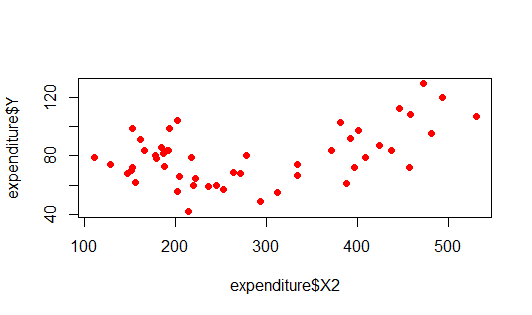
\includegraphics[width=.5\textwidth]{X2_Y}\hfill
		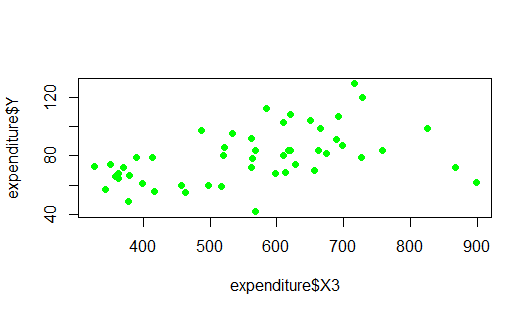
\includegraphics[width=.5\textwidth]{X3_Y}\hfill
		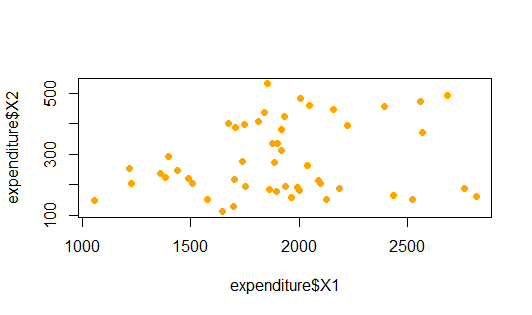
\includegraphics[width=.5\textwidth]{X1_X2}\hfill
		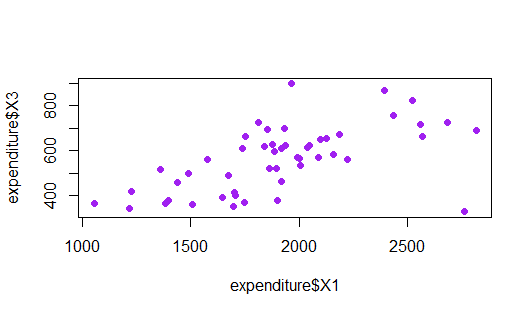
\includegraphics[width=.5\textwidth]{X1_X3}\hfill
		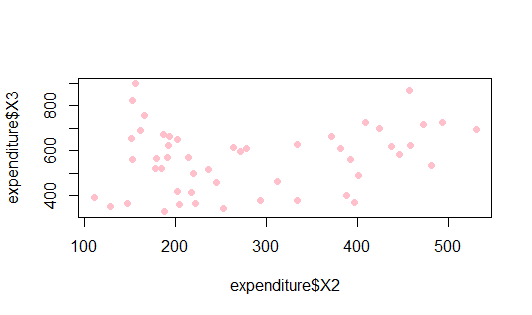
\includegraphics[width=.5\textwidth]{X2_X3}\hfill
		
	\item \textbf{For the plot of \colorbox{blue}{X1 and Y} we see a positive correlation. It looks somewhere in the middle of strong and weak}
	
	\item \textbf{For the plot of \colorbox{red}{X2 and Y}, the graph is somewhat u-shaped, so neither positive or negative}
	
	\item \textbf{For the plot of\colorbox{green}{X3 and Y}, the graph is positive and looks weak}
	
	\item \textbf{For the plot of \colorbox{orange}{X1 and X2}, the graph is positive and looks weak}
	
	
	
	\item \textbf{For the plot of \colorbox{Orchid}{X1 and X3}, the graph is positive and looks somewhere between weak and strong}
	
	\item \textbf{For the plot of \colorbox{pink}{X1 and X2}, the graph is positive and looks weak}
\end{itemize}
	

\vspace{.5cm}
\item
Please plot the relationship between \emph{Y} and \emph{Region}? On average, which region has the highest per capita expenditure on housing assistance?
\vspace{0cm}


 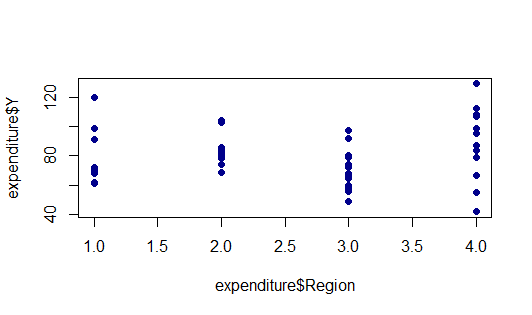
\includegraphics[width=.8\textwidth]{Y_Region}\hfill
		


	\begin{itemize}
		
		\item \textbf{Here is my code for the creating and saving the above plot:}
		
		\lstinputlisting[language=R, firstline=213, lastline=217]{PS01.mine.R}
		
		\item \textbf{I found which region has the highest capita expenditure on housing assistance by making 4 new variables, one for each region. Then I made 4 more variables computing the mean of each region. From this I could see that \colorbox{yellow}{Region 4 (West) had the highest per capita expenditure} \newline \colorbox{yellow}{on housing assistance of 88.31} (rounded to 2 decimal places)}
		
		\item \textbf{Then I put these means into one variable and I plotted it. Results are below my code:}
		
			\lstinputlisting[language=R, firstline=219, lastline=235]{PS01.mine.R}
	\end{itemize}
	
	 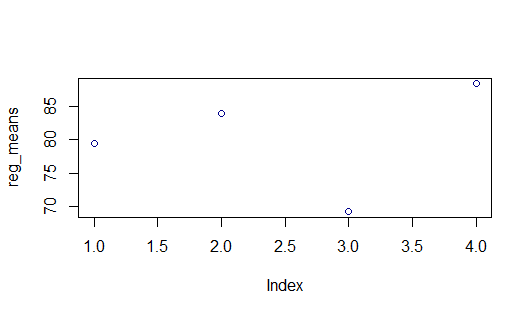
\includegraphics[width=.8\textwidth]{reg_means}\hfill
	
\item
Please plot the relationship between \emph{Y} and \emph{X1}? Describe this graph and the relationship. Reproduce the above graph including one more variable \emph{Region} and display different regions with different types of symbols and colors.


\begin{itemize}
	
	\item \textbf{First I used base r plot and I used code from} \href{https://hbctraining.github.io/Intro-to-R/lessons/basic_plots_in_r.html#:~:text=Basic%20plots%20in%20R,function%20for%20plotting%20x%2Dy%20data.}{this website} 
	\textbf{and my code is as follows:}
	
		\lstinputlisting[language=R, firstline=246, lastline=254]{PS01.mine.R}
		
	\item \textbf{My plot for this is below}
	
\end{itemize}

 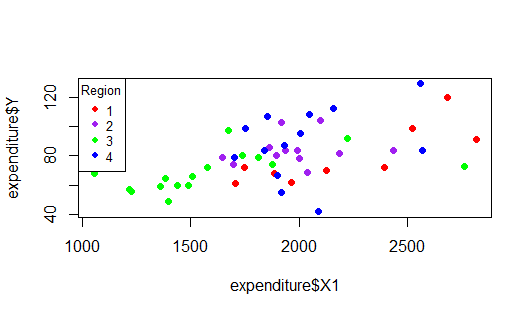
\includegraphics[width=.6\textwidth]{base_r_reg_x1_y}\hfill
 
 \begin{itemize}
 	\item \textbf{But, this only allowed me to change the colors for each region when I wanted to change the shape also. I tried to find a response for this on google and had no luck, so instead I used ggplot. To do so, I first loaded tidyverse:}
 	
 		\lstinputlisting[language=R, firstline=260, lastline=260]{PS01.mine.R}
 		
 	\item \textbf{Then, I used code from coding camp but also used some code from} \href{https://sscc.wisc.edu/sscc/pubs/dvr/three-variables.html}{here} \textbf{to get this code below:}
 	
 		\lstinputlisting[language=R, firstline=264, lastline=272]{PS01.mine.R}
 		
 	\item \textbf{The result is here:}
 	
 	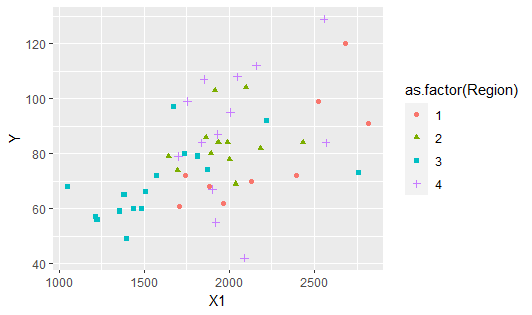
\includegraphics[width=.8\textwidth]{ggplot_reg_x1_y}\hfill
 	
 \end{itemize}


\end{itemize}


\end{document}
